\documentclass[aspectratio=169]{beamer}

% arara: pdflatex 
% arara: biber
% arara: pdflatex
% arara: pdflatex
% arara: clean: {extensions: [aux, bbl, out, toc, blg, thm, log, bcf, snm, nav]}

\usetheme[lightmode, showmaxslides]{pureminimalistic} %darkmode vs lightmode

% *****************************************************************
% Classic
% *****************************************************************
\usepackage[english]{babel}
\usepackage[utf8]{inputenc}
\usepackage[T1]{fontenc}
\usepackage{hyperref}


% ********** Basic supplementray materials
% \usepackage{hvfloat}  % rotation of caption
% \usepackage{rotating}  % allow complete rotation
\usepackage{soul}  % strikethrough text
\usepackage[normalem]{ulem}  % underline text
\usepackage{xcolor}  % color 
% **********


% ********** Maths packages
\usepackage{amssymb,amsmath}
\usepackage{graphicx}
% \usepackage{tikz}
% **********


% ********** Table packages
\usepackage{array}
\usepackage{booktabs}
\usepackage{colortbl}  % color cells
% \usepackage{longtable}
\usepackage{siunitx}
% \usepackage{tabu}
% \usepackage{threeparttable} 
% **********


% ********** Icones packages
\usepackage{fontawesome}
\usepackage{orcidlink}
\usepackage{tfrupee}
% **********


% ********** Define color + color configuration
\definecolor{NUred}{RGB}{213, 17, 45}
\definecolor{NUblue}{RGB}{0, 59, 113}
\definecolor{UBbrown}{RGB}{48, 33, 25}
\definecolor{UBblue}{RGB}{0, 158, 214}
\definecolor{ODRIISdarkgreen}{RGB}{80,151,68}
\definecolor{ODRIISlightgreen}{RGB}{164,204,76}
\definecolor{ODRIISbrick}{RGB}{197,102,63}
\definecolor{lightgray}{HTML}{A9A9A9}
\definecolor{lightgray2}{RGB}{113,113,113}
% **********
\hypersetup{colorlinks,linkcolor={lightgray2},citecolor={ODRIISdarkgreen},urlcolor={ODRIISdarkgreen}}
%\renewcommand{\beamertextcolor}{}
%\renewcommand{\beamerbgcolor}{}
%\renewcommand{\beamerfootertextcolor}{}
\renewcommand{\beamertitlecolor}{ODRIISbrick}
\setbeamercolor{button}{bg=ODRIISdarkgreen,fg=ODRIISlightgreen!10}
% **********





% *****************************************************************
% Pureminimalistic configuration
% *****************************************************************
\renewcommand{\logotitle}{\vspace*{-20mm}\hspace*{-10.1mm}
\includegraphics[width=\paperwidth]{Beamer_theme/header2.jpeg}}
\renewcommand{\logoheader}{\vspace{0em}}
\renewcommand{\logoheader}{\vspace{0em}}
\renewcommand{\logofooter}{\href{https://odriis.hypotheses.org/}{
\includegraphics[width=.6\linewidth]{Beamer_theme/odriis_long.png}}}



% *****************************************************************
% Caption configuration
% *****************************************************************
\usepackage{caption}  % custom caption

\captionsetup{
font=small,
skip=1em,
labelfont={bf},
justification=centering,
singlelinecheck=false,
%textfont={bf,it},
%labelsep=endash,
%tableposition=top,
}






% *****************************************************************
% Appendix
% *****************************************************************
\usepackage{appendixnumberbeamer}
\renewcommand{\appendixname}{\texorpdfstring{\translate{appendix}}{appendix}}





% *****************************************************************
% Bibliography
% *****************************************************************

% ********** Bibtex
% \usepackage[doi, natbibapa]{apacite}
% \renewcommand\bibliographytypesize{\tiny}
% \let\realcitep\citep
% \renewcommand*{\citep}[1]{{\small\realcitep{#1}}}
% \let\realcite\cite
% \renewcommand*{\cite}[1]{{\small\realcite{#1}}}
% ********** 


% ********** Biblatex
\usepackage[
natbib=true,
backend=biber,
style=trad-abbrv,
sorting=none, %nyt
]{biblatex}
% **********
\renewcommand*{\bibfont}{\footnotesize}





% *****************************************************************
% Bigcenter
% *****************************************************************
\makeatletter
\newskip\@bigflushglue \@bigflushglue = -100pt plus 1fil
\def\bigcenter{\trivlist \bigcentering\item\relax}
\def\bigcentering{\let\\\@centercr\rightskip\@bigflushglue%
\leftskip\@bigflushglue
\parindent\z@\parfillskip\z@skip}
\def\endbigcenter{\endtrivlist}
\makeatother






% *****************************************************************
% Box creation
% *****************************************************************
\usepackage[most]{tcolorbox}

\newtcolorbox{greenbox}[2][]{colback=ODRIISlightgreen!10,colframe=ODRIISlightgreen!10,coltitle=black,colbacktitle=ODRIISdarkgreen!20,title={#2},#1}
\newtcolorbox{brickbox}[1][]{colback=ODRIISbrick!10,colframe=ODRIISbrick!10,#1}






% *****************************************************************
% Section page
% *****************************************************************
\newcommand{\secttitle}[1]{
\begin{columns} 
\begin{column}{.4\textwidth}
\vspace*{-0mm}\hspace*{-10.1mm}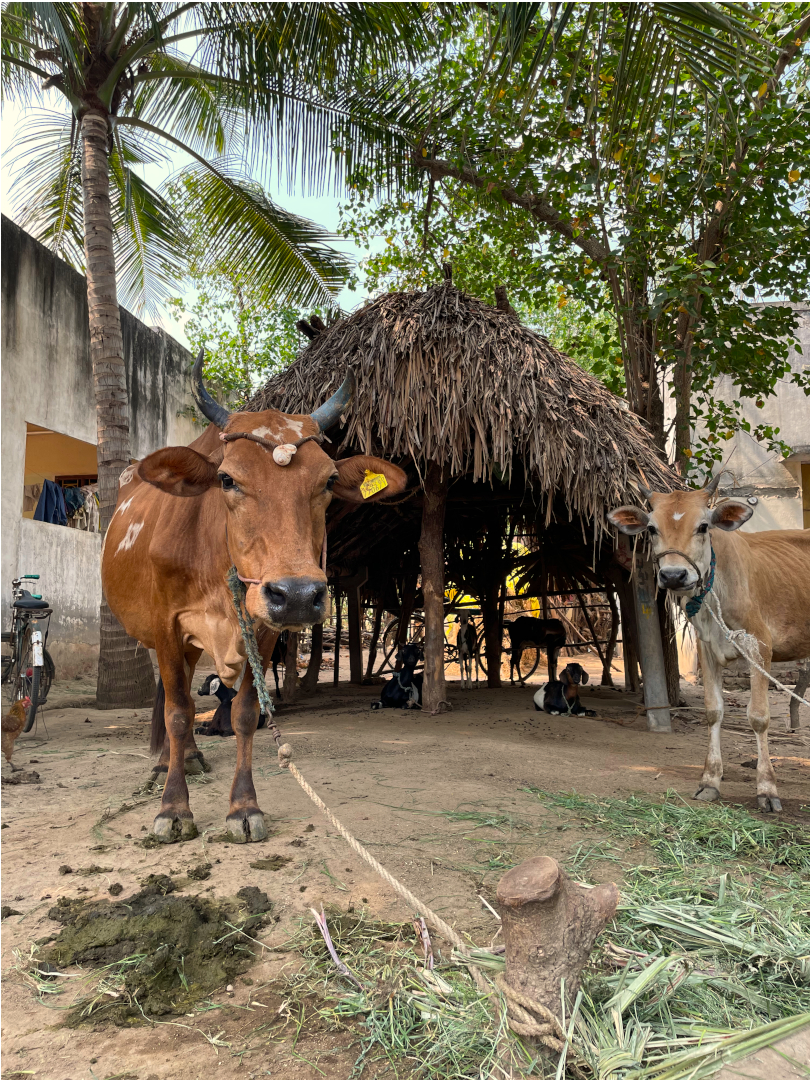
\includegraphics[height=\paperheight]{Beamer_theme/cow.jpeg}
\end{column}
\begin{column}{.6\textwidth}
\vfill
\begin{tcolorbox}[colback=ODRIISlightgreen!20,colframe=ODRIISlightgreen!20,box align=center,halign=center,valign=center]
{\LARGE \textcolor{ODRIISbrick}{#1}}
\end{tcolorbox}
\vfill
\end{column}
\end{columns}
}






% *****************************************************************
% Table
% *****************************************************************

% ********** Stars
\newcommand{\sym}[1]{\rlap{#1}}% Thanks to David Carlisle
% **********


% ********** Insert the table
\newcommand{\inserttable}[3]{
\resizebox{#3}{!}{
\begin{tabular}{#2}
\toprule
\input #1
\bottomrule
\end{tabular}
}
}
% **********


% ********** Source
\newcommand{\bottomtext}[1]{\vspace{-1.5ex}\captionsetup{justification=centering,font=footnotesize,singlelinecheck=false}\caption*{\hangindent=1.5em #1}}
\newcommand{\bottomnote}[1]{\bottomtext{\textit{Note}:~#1}}
\newcommand{\source}[1]{\bottomtext{\textit{Source}:~#1}}
\newcommand{\starnote}{\bottomtext{* p < 0.1, ** p < 0.05, *** p < 0.01. Standard error in parentheses.}}
% **********


% ********** siunitx config
\sisetup{
detect-mode,
tight-spacing= true,
group-digits= false ,
input-signs= ,
input-symbols= ( ) [ ] - + *,
input-open-uncertainty=,
input-close-uncertainty=,
table-align-text-post=false
}
% **********


% ********** Linebreak in cell
\newcommand{\specialcell}[2][c]{\begin{tabular}[#1]{@{}c@{}}#2\end{tabular}}
% **********


% \makeatletter
% \AddToHook{env/tabular/begin}{\let\input\@@input}
% \makeatother




% *****************************************************************
% Personnal cmd
% *****************************************************************
\newcommand{\jati}[1]{\textit{j\={a}ti{#1}}}

\newcommand\dev[1]{\textbf{\textcolor{red}{#1}}}

\newcommand{\ie}{i.e.}
\newcommand{\sd}{standard deviation}
\newcommand{\pp}{percentage points}
\newcommand{\aebe}{all else being equal}
\newcommand{\Aebe}{All else being equal}
\newcommand{\ote}{other things equal}
\newcommand{\Ote}{Other things equal}
\newcommand{\cl}{confidence level}
\newcommand{\lit}{\dev{literature}}
\newcommand{\PTCS}{PT\&CS}

\newcommand{\key}[1]{\underline{\textsc{#1}}}
\newcommand{\data}[1]{\textbf{\underline{Data #1:}}~}


% ********** Symbol shortcuts
\def\@fnsymbol#1{\ensuremath{\ifcase#1\or *\or \dagger\or \ddagger\or
   \mathsection\or \mathparagraph\or \|\or **\or \dagger\dagger
   \or \ddagger\ddagger \else\@ctrerr\fi}}
   
\makeatletter
\newcommand{\ssymbol}[1]{^{\@fnsymbol{#1}}}
\makeatother
% **********

% ********** Bibliography
\addbibresource{Ref_Arnaud.bib}
% ********** 

\setbeamercovered{transparent}






% *****************************************************************
% Title
% *****************************************************************
\title[Psychology of debt]{\textsc{Psychology of Debt in Rural South India}}
\author[A. Natal and C.J. Nordman]{\textcolor{ODRIISdarkgreen}{Arnaud Natal\orcidlink{0000-0003-1301-2281}} \textcolor{ODRIISlightgreen}{\scriptsize Univ. Bordeaux} \\ 
\textcolor{ODRIISdarkgreen}{Christophe J. Nordman} \textcolor{ODRIISlightgreen}{\scriptsize LEDa-DIAL, IRD, PSL University and IFP}} 
\institute{\\ ICDE | \small \today} 


% ******************************************************************
\begin{document}

\maketitle



% *******************
\begin{frame}{Motivation}
Increasing interest in:
\begin{itemize}
	\item Personality traits and cognitive skills (\PTCS~) \citep{Almlund2011};
	\item Household finance \citep{Gomes2021}.
	\item[$\rightarrow$] in the USA \citep{Agarwal2013};
	\item[$\rightarrow$] in the UK \citep{Brown2014}.
\end{itemize}

Developping countries remains a blind spot, while:
\begin{enumerate}
	\item Credit as exit to poverty \citep{Burgess2005};
	\item Informal debt \citep{Badarinza2019}.
\end{enumerate}

\begin{brickbox}
\centering Fill this gap by considering the case of rural South India.
\end{brickbox}

\end{frame}
% *******************






% *******************
\begin{frame}{Questioning and contributions}

We explore the relationship between: 

\begin{tabular}{lcl}
\PTCS~ & and & recourse, \\
       &     & negotiation, \\
       &     & management of debt. \\
\end{tabular}

While taking into account the weight of \textit{social identity} (sex and caste).

\begin{greenbox}{Contributions:}
\begin{enumerate}
\item Household indebtedness in developing countries \citep{Badarinza2019};
\item \PTCS~ and economic outcomes \citep{Borghans2008};
\item \PTCS~ on negotiation process \citep{Elfenbein2015};
\item Social identity in economic choices \citep{Benjamin2010}.
\end{enumerate}
\end{greenbox}

\end{frame}
% *******************




% *******************
% \begin{frame}{Big-5 taxonomy \& cognitive skills}

% Big-5 personality traits:
% \begin{itemize}
	% \item Emotional stability: tendency to experience negative emotions
	% \item Extraversion: tendency to seek stimulation and company
% from others
	% \item Openness to experience: capacity to be creative and unstructured
	% \item Agreeableness: perceptions of others that are caring, compassionate, and altru-
% istic
	% \item Conscientiousness: capacity to display self-discipline, act dutifully, and
% strive for achievement against measures or outside expectations
% \end{itemize}

% Cognitive skills:
% \begin{itemize}
	% \item Math score;
	% \item Literacy score;
	% \item Raven score. 
% \end{itemize}

% \end{frame}
% *******************





% *******************
% \begin{frame}{Main results:}

% \begin{tabular}{lll}
% \midrule
% Traits					& Relation		& Aspect of debt \\
% \midrule
% Openness-extraversion 	& Liability		& Negotiation	\\
% Openness-extraversion 	& Liability		& Management	\\
% Conscientiousness		& Asset	& Negotiation	\\
% Conscientiousness		& Asset	& Management	\\
% Cognitive skills		& Asset	& Management	\\
% \midrule
% \end{tabular}


% + Use of personality traits and cognitive skills as a way to overcome the weight of social identity for the female.

% \end{frame}
% *******************






% *******************
\begin{frame}[plain,noframenumbering]

\secttitle{Theoretical framework}

\end{frame}
% *******************




% *******************
\begin{frame}{Theoretical framework I}

Increasing of debt in rural India since the 1980's \citep{Rajakumar2019}:
\begin{itemize}
\item Incidence goes from 19 to 32\%, 
\item but largely underestimated \citep{Jones1994}: 80-90\%.
\item Amount goes from 283 to 33,000.
\item[$\rightarrow$] Good debt management is essential.% and literature highlights individual psychology in debt management \citep{Amar2011}.
\end{itemize}


Especially to the disadvantage of \textit{Dalits} \citep{Kumar2013}, and females \citep{Reboul2021}.

%Recent crises are fuelling this increase and widening inequalities \citep{GuerinDemo2017,Guerin2022}.
\begin{itemize}
\item[$\rightarrow$] Need to take into account the social identity.
\end{itemize}

\end{frame}
% *******************




% *******************
\begin{frame}{Theoretical framework II}

The cornerstone of debt in India is its social meaning \citep{Guerin2014a}
\begin{itemize}
\item Set of rights and obligations that links borrowers (Br) and lenders (Lr) into a strong relationship.
\item Consequences in terms of social belonging, status, and dignity.
\item Not fixed but continuously bargained and negotiated.
\item[$\rightarrow$] Expression of individual differences in the negotiation process \citep{Elfenbein2015}.
\end{itemize}

\end{frame}
% *******************






% *******************
\begin{frame}[plain,noframenumbering]

\secttitle{Data \& methodology}

\end{frame}
% *******************





% *******************
\begin{frame}{Data I}

\href{https://neemsis.hypotheses.org/}{NEEMSIS} dataset from the Observatory of Rural Dynamics and Inequalities in South India: \href{https://odriis.hypotheses.org/}{https://odriis.hypotheses.org}
\begin{itemize}
\item Follow-up the RUME survey implemented in 2010 in 10 villages of rural Tamil Nadu.
\item NEEMSIS-1 (2016-17) and NEEMSIS-2 (2020-21) used here are the second and third waves
of a the longitudinal household survey.
\item[$\rightarrow$] NEEMSIS-1 consists of 492 HH of which 485 are in panel setting with NEEMSIS-2.
\end{itemize}

2 HH members (the head and one younger randomly selected on a criterion of age), called ``egos'' are directly addressed an individual questionnaire which provide information on \PTCS~.
\begin{itemize}
\item[$\rightarrow$] Total of 835 individuals ``egos'' in panel setting (2016-17 \& 2020-21).
\end{itemize}

\end{frame}
% *******************



% *******************
% \begin{frame}{Data II}

% Data on indebtedness are notoriously difficult to collect and prone to underreporting due to recall issues and social desirability biases \citep{Karlan2008}.
% \begin{itemize}
% \item[$\rightarrow$] 99\% of HH are indebted in NEEMSIS-1 while nationwide AIDIS data report an incidence of 30\% in rural Tamil Nadu in 2012 \citep{NSSO2014}.
% \end{itemize}

% \begin{brickbox}
% Moreover, NEEMSIS dataset have the \underline{rare} and \underline{valuable} advantage of recording debt at the individual level.
% \end{brickbox}

% \end{frame}
% *******************



% *******************
\begin{frame}{Construction of \PTCS~ variables I}

\begin{brickbox}
Exogeneity of \PTCS~ assumed thank to the stability over time.
\begin{itemize}
\item Our data suggest stability for a minor part of the population.
\item[$\rightarrow$] We use 2016-17 measures of \PTCS~ on debt in 2020-21 \citep{Anger2017a}.
\end{itemize}
\end{brickbox}

\vspace*{0.5em}

\textbf{Cognitive skills in 2016-17 ~~---}
\vspace*{0.2em}

\begin{tabular}{llll}
• Literacy score 	& by $\sum$ of 4 dummies questions \\
• Numeracy score 	& by $\sum$ of 4 dummies questions \\
• Raven score 	& by $\sum$ of 36 dummies questions	\\
\end{tabular}

%\vspace*{0.2em}
%We standardise resulting scores to ensure comparability.

\end{frame}
% *******************




% *******************
\begin{frame}{Construction of \PTCS~ variables II}
\label{frame:construction2}

\textbf{Personality traits in 2016-17 ~~---}
\vspace*{0.2em}

A set of 35 affirmative questions \citep{John1999}.

~ \hfill \hyperlink{frame:questions}{\beamerbutton{questions}} +  \hyperlink{frame:compconst}{\beamerbutton{construction}} \hfill ~

\begin{itemize}
\item[$\rightarrow$] Correction of the acquiescence bias; 
\item[$\rightarrow$] Factor analysis by principal component with oblique quartimin rotation \citep{Laajaj2019b}.
\item[F1] as emotional stability (McDonald's $\omega=0.88$);
\item[F2] as conscientiousness (McDonald's $\omega=0.84$);
\item[F3] as openness-extraversion (McDonald's $\omega=0.81$);
\item[\st{F4}]\st{as weak emotional stability (McDonald's $\omega=0.54$);}
\item[F5] as agreeableness (McDonald's $\omega=0.56$).
\end{itemize}

\end{frame}
% *******************




% *******************
% \begin{frame}{Construction of \PTCS~ variables III}

% Resulting factors are similar to the Big-5 taxonomy with satisfactory internal consistencies:

% \begin{itemize}
% \item Factor 1 as emotional stability (McDonald's $\omega=0.88$);
% \item Factor 2 as conscientiousness (McDonald's $\omega=0.84$);
% \item Factor 3 as openness-extraversion (McDonald's $\omega=0.81$);
% \item \st{Factor 4 as weak emotional stability (McDonald's $\omega=0.54$);}
% \item Factor 5 as agreeableness (McDonald's $\omega=0.56$);
% \end{itemize}

% \begin{brickbox}
% We run an univariate OLS regressions with \PTCS~ as endogenous variables and age as exogenous variable to remove the effect of age on \PTCS~ \citep{Brown2014}.

% We standardised the residuals and used them as age-effect-free \PTCS~.
% \end{brickbox}

% \end{frame}
% *******************



% *******************
\begin{frame}{Measures of debt}

\resizebox{0.9\columnwidth}{!}{%
\begin{tabular}{llll}
\textbf{Recourse ~~---} & & & \\
\midrule
Prob. individual is in debt  & Dum. & & \\
Total amount of debt &	Cont.  & (-) CO. (+) ES. & \citep{Brown2014} \\
& & & \\
\textbf{Negotiation ~~---} & & &  \\
\midrule
Interest of debt service ratio & Cont. &  (+) EX. (+) AG.& \citep{Elfenbein2015}  \\
Prob. Lr provide finan. support & Dum.  & (-) EX. (-) AG. & \citep{Elfenbein2015} \\
Prob. Br no need to provide services & Dum. & (-) EX. (-) AG. & \citep{Elfenbein2015} \\
& & & \\
\textbf{Management ~~---} & & &  \\
\midrule
Prob. Br re-borrow to repay & Dum. & (-) CO. &  \citep{Donnelly2012} \\
Prob. Br have a pb to repay & Dum. &  (-) CO. & \citep{Donnelly2012} \\
\end{tabular}
}

\end{frame}
% *******************




% *******************
\begin{frame}{Empirical strategy I}
\label{frame:empirical1}

\begin{brickbox}
Our analysis faces non-random sample selection issues because the sample is restricted to those who declared a non-zero and non-missing debt.
\begin{itemize}
\item Heckman procedure not possible because we do not have exclusion restriction variables.
\item[$\rightarrow$] We exclude non-participants to debt \citep{Rio2006}.
\end{itemize}
\end{brickbox}

\begin{align}
\label{eq:reg1} Y_{i} & = \beta_{0}+PTCS'_{i}*\beta_{1}+X'_{i}*\beta_{2}+\epsilon_i
\end{align}

$X'$ individual and household level \hyperlink{frame:control}{\beamerbutton{controls}} + cluster std err. at HH level because obersations within HH are not i.i.d.

\end{frame}
% *******************






% *******************
\begin{frame}{Empirical strategy II}
To take into account the weight of social identity, we use interaction variables:

\begin{align}
\label{eq:reg2} Y_{i} & = \beta_{0}+PTCS'_{i}*\beta_{1}+X'_{i}*\beta_{2}+PTCS'_{i}*Sex_{i}*\beta_{3}+\epsilon_i  \\ 
\label{eq:reg3} Y_{i} & = \beta_{0}+PTCS'_{i}*\beta_{1}+X'_{i}*\beta_{2}+PTCS'_{i}*Caste_{i}*\beta_{3}+\epsilon_i  \\ 
\label{eq:reg4} Y_{i} & = \beta_{0}+PTCS'_{i}*\beta_{1}+X'_{i}*\beta_{2}+PTCS'_{i}*Sex_{i}*Caste_{i}*\beta_{3}+\epsilon_i 
\end{align}

\begin{greenbox}{Interpretation \citep{Buis2010}}
ME at representative values of sex and caste.
All other covariables at the mean. 
Allows us to create 9 subgroups of ME. 
\begin{itemize}
\item[$\rightarrow$] How the effects of \PTCS~ vary according to social identities?
\end{itemize}
\end{greenbox}

\end{frame}
% *******************







% *******************
\begin{frame}[plain,noframenumbering]

\secttitle{Descriptive statistics}

\end{frame}
% *******************





% *******************
\begin{frame}{Household level statistics IV}

% \begin{figure}[h]
% \centering
% \includegraphics[scale=0.7]{INPUT/Kernel_PTCS}
% \source{NEEMSIS-1 (2016-17); author's calculations.}
% \end{figure}


\end{frame}
% *******************







% *******************
\begin{frame}[plain,noframenumbering]

\secttitle{Results}

\end{frame}
% *******************








% *******************
\begin{frame}{Management II}

% \begin{table}[!h]
% \centering
% \caption{ME of the probability to have problem to repay the debt}
% \inserttable{INPUT/ame_dummyproblemtorepay.tex}{lcccccccccccc}{0.8\columnwidth}
% \starnote
% \source{NEEMSIS-1 (2016-17) \& NEEMSIS-2 (2020-21); author's calculations.}
% \end{table}

\end{frame}
% *******************







% *******************
\begin{frame}[plain,noframenumbering]

\secttitle{Discussion}

\end{frame}
% *******************



% *******************
\begin{frame}{Discussion I}

\textbf{Recourse ~~---}
\begin{itemize}
\item[$\rightarrow$] Overall, \PTCS~ play a limited role.
\end{itemize}


\textbf{Negotiation ~~---}
\begin{itemize}
\item \citep{Barry1998} extraversion tends to be a liability:
\item Dalit females and ISR.
\item non-Dalit males and provide services in return for the loan.
\item low extroversion tend to be calmer
\item An individual with low openness to experience tend to be more suspicious which can lead him to ask himself more questions to know where he is going in the negotiation and thus better ``defend'' his interests.
\item low openness to experience is associated with more “simplicity” and a more prominent ``direct side'' which can make it easier to defend it is own interests in a negotiation process.
\end{itemize}


\end{frame}
% *******************




% *******************
\begin{frame}[plain,noframenumbering]

\secttitle{Conclusion}

\end{frame}
% *******************







% *******************
\section*{References}
\begin{frame}[noframenumbering, allowframebreaks]{References}

\printbibliography[title={References},heading=none]

\end{frame}
% *******************


% *******************
\begin{frame}[noframenumbering]{Controls I}
\label{frame:control}

\hyperlink{frame:empirical1}{\beamerbutton{back}}

\begin{greenbox}{Individual level controls}
Age; age square; sex; dummy variable which takes 1 if individual is the household head, 0 otherwise; main occupation defines as the most time-consuming activity; dummy variable which takes 1 if individuals received formal education through school, 0 otherwise and a dummy variable which take 1 if individual is married, 0 otherwise.
Also, dummy variable which takes 1 if individual is indebted in 2016-17, 0 otherwise.
\end{greenbox}

\end{frame}
% *******************


% *******************
\begin{frame}[noframenumbering]{Controls II}
\label{frame:control}

\hyperlink{frame:empirical1}{\beamerbutton{back}}

\begin{greenbox}{Household level controls}
caste (Dalit or not); monetary value of assets (include gold; land; house; livestock; agricultural equipment and consumption good); total annual income; household size; shock exposure (dummy variable which takes 1 if the household experienced a marriage of at least one of the household members between 2016-17 and 2020-21 or/and whether the household has been surveyed after the demonetisation of November 2016, 0 if not). 
We control for the ``degree'' of exposition of COVID-19.
We add dummy variable which takes 1 if the household had to sell assets to cope with the difficulties of the lockdown.
\end{greenbox}

\end{frame}
% *******************



% *******************
\begin{frame}[noframenumbering]{Controls III}
\label{frame:control}

\hyperlink{frame:empirical1}{\beamerbutton{back}}

\begin{greenbox}{Specific control variables}
Negotiation: percentage of loans from an individual of the same sex and percentage from an individual of the same caste.
\begin{itemize}
\item[$\rightarrow$] when the Lr and the Br have the same sex or caste, negotiations can be easier. We believe that caste solidarity \citep{Guerin2021b} can facilitate negotiation.
\end{itemize}

Management: total amount of debt.
\begin{itemize}
\item[$\rightarrow$] the higher the debt, the more difficult it is to manage.
\end{itemize}
\end{greenbox}

\end{frame}
% *******************








% *******************
\begin{frame}[noframenumbering]{Contacts}
 
\begin{columns}
\begin{column}{0.5\textwidth}
\begin{center}
Arnaud Natal, \\
\textcolor{ODRIISlightgreen}{\footnotesize{Univ. Bordeaux, CNRS, BSE, UMR 6060}} \\
\href{https://orcid.org/0000-0003-1301-2281}{\footnotesize{orcid.org/0000-0003-1301-2281}} \\
\href{mailto:arnaud.natal@u-bordeaux.fr}{\footnotesize{arnaud.natal@u-bordeaux.fr}} \\
\href{https://arnaudnatal.github.io}{\footnotesize{arnaudnatal.github.io}}
\end{center}
\end{column}
\begin{column}{0.5\textwidth}  %%<--- here
\begin{center}
Christophe J. Nordman, \\
\textcolor{ODRIISlightgreen}{\footnotesize{LEDa-DIAL, IRD, PSL University and IFP}}
\href{mailto:nordman@dial.prd.fr}{\footnotesize{nordman@dial.prd.fr}} \\
\end{center}
\end{column}
\end{columns}


\vskip0ptplus1filll\relax
\begin{center}
\small Credit images: BTS. April 27, 2021. Manam.
\end{center}

\end{frame}
% *******************





\end{document}





% *******************
%\begin{frame}[plain, shrink=2]{Correction 1 \citep{Rammstedt2013}}
%\begin{figure}[htpb]
%\centering
%\includegraphics[scale=1]{INPUT/boxplotars.pdf}
%\end{figure}
%\end{frame}
% *******************





% *******************
%\begin{frame}[plain, shrink=2]{Résultats}
%\input{INPUT/AME_indebt.tex}
%\end{frame}
% *******************

% *******************
% \begin{frame}{Figures}
%     \begin{figure}[H]
%         \centering
%         \begin{columns}[T]
%             \begin{column}{.3\linewidth}
%                 \includegraphics[width=\linewidth]{example-image-a}
%                 \caption{Example A}
%             \end{column}
%             \begin{column}{.3\linewidth}
%                 \includegraphics[width=\linewidth]{example-image-b}
%                 \caption{Example B}
%             \end{column}
%         \end{columns}
%     \end{figure}
% \end{frame}
% *******************